\documentclass{article}
\usepackage{amsmath}
\usepackage{amsfonts}
\usepackage{mathtools}
\usepackage{graphicx}
\usepackage{subfigure}
\usepackage{url}
\usepackage{fullpage}
\usepackage{color}
\usepackage{mathrsfs}
\usepackage{natbib}
\usepackage{hyperref}
\usepackage{mathptmx}
\usepackage[figuresright]{rotating}
\usepackage{threeparttable}
%
%
\usepackage[T1]{fontenc}
\usepackage[utf8]{inputenc}
\usepackage{authblk}
%
%
\title{Advancing Treatment of Retinal Disease through \emph{in silico} Trials}
\author[1,2]{R\'{e}mi Hernandez\footnote{E-mail address: remi.hernandez@liverpool.ac.uk (R\'{e}mi Hernandez)}}
\author[3]{Paul A. Roberts\footnote{E-mail address: p.a.roberts@univ.oxon.org (Paul A. Roberts)}}
\author[1,2]{Wahbi K. El-Bouri\footnote{E-mail address: w.el-bouri@liverpool.ac.uk (Wahbi K. El-Bouri)}}
\affil[1]{Liverpool Centre for Cardiovascular Science, University of Liverpool and Liverpool Heart \& Chest Hospital Liverpool, UK}
\affil[2]{Department of Cardiovascular and Metabolic Medicine, University of Liverpool, UK}
\affil[3]{Centre for Systems Modelling and Quantitative Biomedicine, University of Birmingham, Institute of Biomedical Research, Birmingham, B15 2TT, UK}
%
\renewcommand\Authands{ and }
%  
%
\begin{document}
%
%
\date{\vspace{-5ex}}
%
%
\maketitle
%
%
\tableofcontents
%
%
\section{Retinal oxygenation, retinitis pigmentosa \& non-neovascular AMD}\label{Sec_Ox_RP_nnAMD}
%
%
\subsection{Retinal oxygenation}\label{Sec_Oxygen}
%
The retina is one of the most oxygen hungry tissues in the body \citep[per gram of tissue][]{Anderson_1968,Anderson_and_Saltzman_1964,Yu_and_Cringle_2001,W-Wirawan_and_Linsenmeier_2003}. As described in \textcolor{red}{Section \ref{}}, it has a substantial vasculature to meet this need; nonetheless, supply and demand are finely balanced. It is therefore important to understand how this balance is maintained, and the ways in which it may be dysregulated in diseases such as RP and nnAMD (see Sections \ref{Sec_RP} and \ref{Sec_nnAMD}).

Two key techniques are frequently employed to measure retinal oxygenation. First, oxygen-sensitive microelectrodes can be used to measure the partial pressure of oxygen (PO$_2$), creating a spatially detailed profile through the depth of the retinal tissue \citep{Linsenmeier_and_Zhang_2017}. Since this technique is invasive, it can only be employed in animal models. Second, oximetry can be used to measure the oxygen saturation of haemoglobin in the retinal vasculature \citep{Linsenmeier_and_Zhang_2017}. As a non-invasive technique, this can be employed in both animals and humans.

Mathematical modelling of retinal oxygenation has great value. It enables us to get more information out of experimental data (e.g.\ calculating the rate of oxygen consumption of different retinal layers), to predict oxygen profiles in cases where these cannot be measured (e.g.\ in humans) and to determine how variations in retinal physiology or biochemistry may affect oxygen supply (e.g.\ in RP and nnAMD).

A range of mathematical models have been developed to explore various aspects of retinal oxygenation. The most common approach is to model the 1D oxygen profile through the retinal depth using spatial ODE models, accounting for variations in oxygen supply and demand between layers \citep[utilising anywhere between 1 and 8 model layers,][]{Braun_et_al_1995,Cringle_and_Yu_2002,Dollery_et_al_1969,Haugh_et_al_1990,Linsenmeier_1986,Stefansson_1988}. These models have the advantage of being analytically tractable and can easily be fitted to microelectrode data. They can also be extended to incorporate other biomolecules such as neuroglobin, which has been suggested to play a role in enhancing oxygenation by transporting and storing oxygen \citep{Fago_et_al_2004_b,Roberts_et_al_2016a}.

A similarly simple approach is to model each layer as a separate 0D compartment, predicting the evolving oxygen concentration in each compartment using time-dependent ODEs \citep[see][who also model nitric oxide concentrations]{German_et_al_2021}.

More complex models also exist, extending into higher spatial dimensions (2D/3D) and/or incorporating more explicit representations of retinal vasculature, and blood flow mechanics and regulation \citep[see Figure \ref{Fig_Fry2020},][see also Section \ref{Sec_nnAMD} for models relevant to nnAMD]{Aquah_et_al_2021,Arciero_et_al_2021,Causin_et_al_2016,Friedland_1978,Fry_et_al_2018,Fry_et_al_2020,Linsenmeier_and_Zhang_2017,McDougall_et_al_2012,Watson_et_al_2012}. These models are more computationally expensive than those described above; however, they have the advantage of more faithfully representing retinal physiology, and have the potential, in time, to be used in personalised medicine.
%
\begin{figure}
\begin{center}
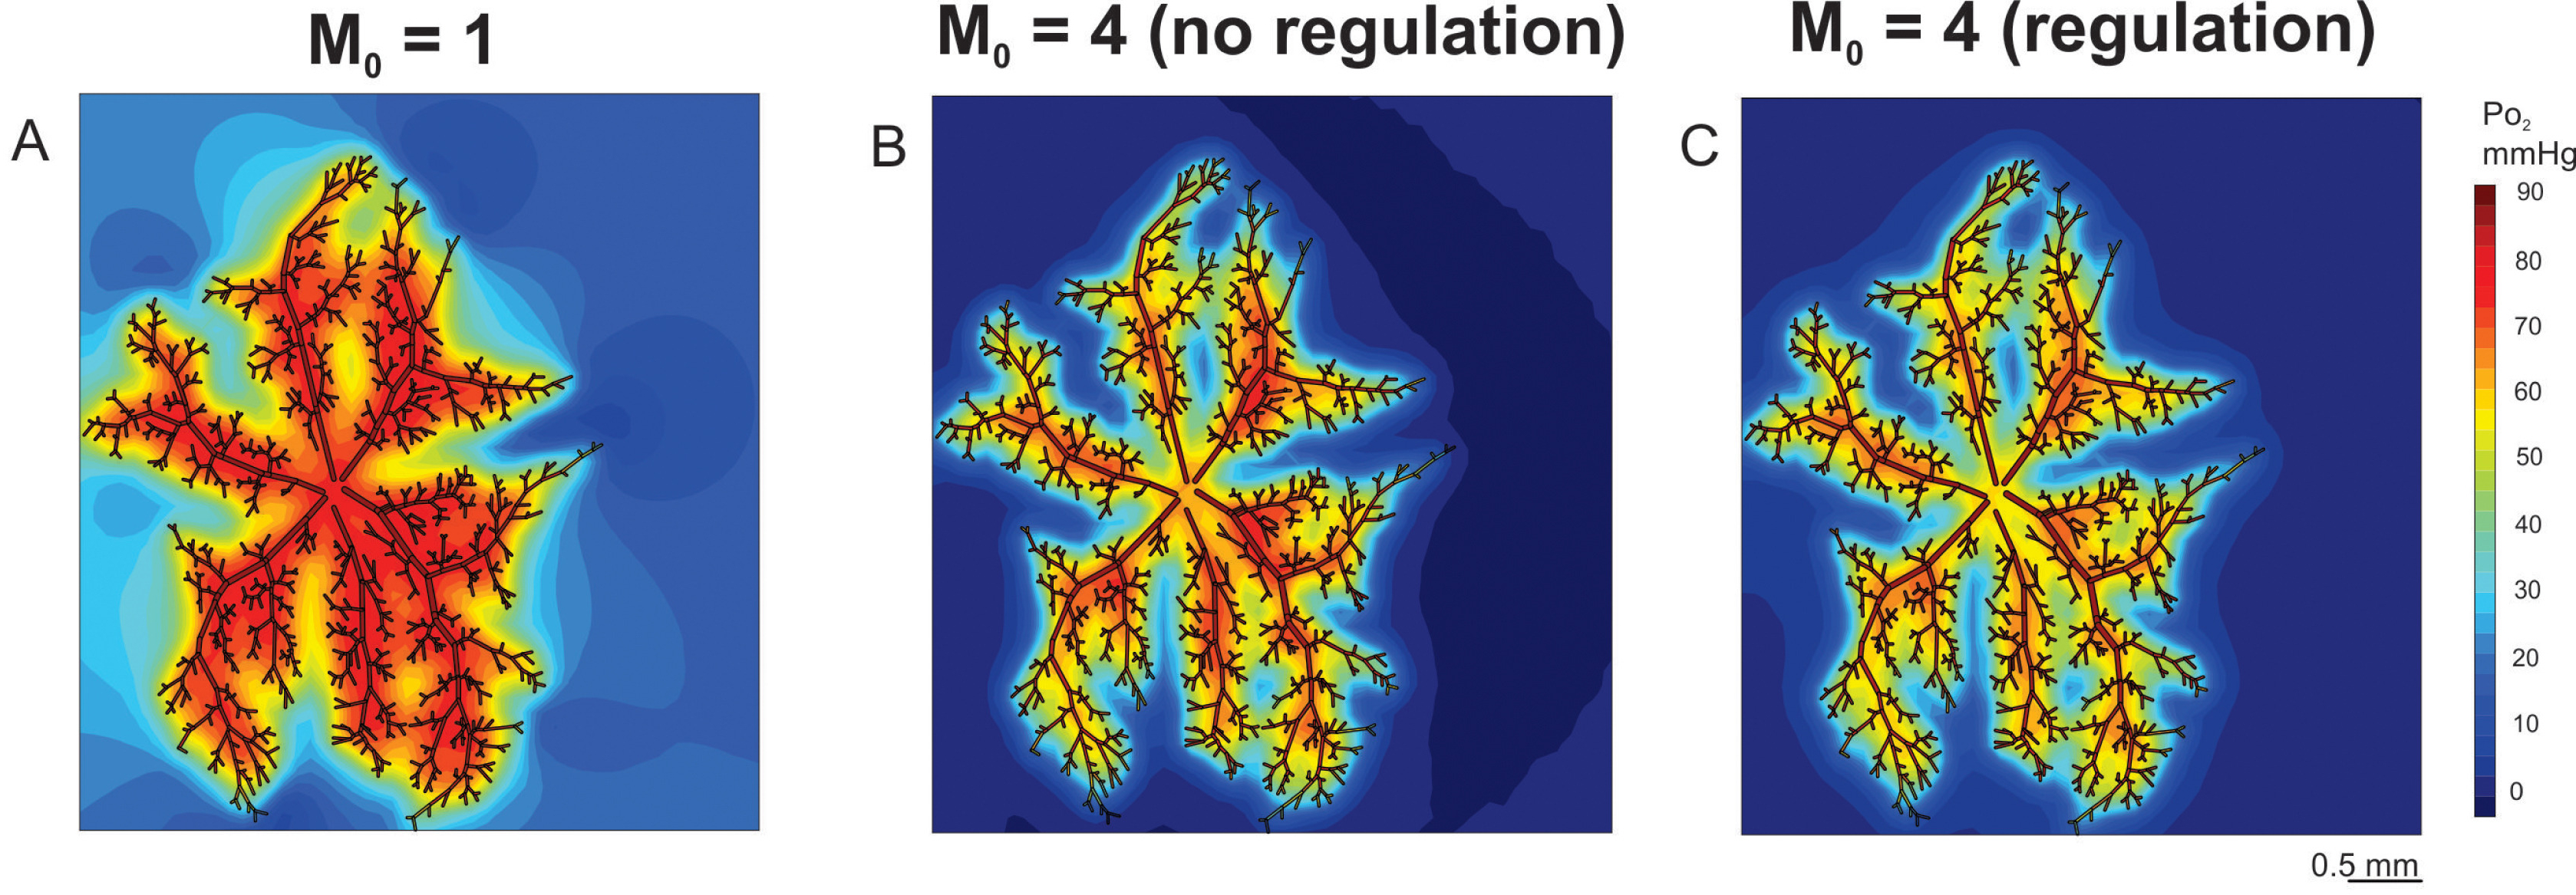
\includegraphics[scale=0.95]{Fry_et_al_2020_Fig_3_ABC}
\end{center}
\caption{Oxygen distribution (PO$_2$) within the arteriolar network and surrounding retinal tissue. Heatmaps are shown for low (A) and high (B and C) tissue oxygen consumption rates, $M_0$ (cm$^3$O$_2$/100cm$^3$/min), both with (C) and without (B) regulation (conducted metabolic response). Figure reproduced, with permission, from \citet{Fry_et_al_2020}.}
\label{Fig_Fry2020}
\end{figure}
%
%
\subsection{Retinitis pigmentosa}\label{Sec_RP}
%
Retinitis pigmentosa (RP) is a term used to denote a group of inherited retinal diseases that result in progressive vision loss \citep{Hamel_2006,Hartong_et_al_2006}. RP typically presents as a rod-cone dystrophy, in which rod photoreceptors malfunction and die before cone photoreceptors, though the term is often used to encompass cone-rod dystrophies, in which cones are affected first, and rarer cases where both rods and cones are affected on a similar timescale \citep{Hamel_2006,Hartong_et_al_2006}. In what follows, we shall focus largely on the rod-cone dystrophy form.

Rods degenerate because either they or the underlying RPE express a mutant gene; however, cones do not typically express a mutant RP gene, so the cause of cone death is unclear \citep{Daiger_et_al_2007,Ferrari_et_al_2011,Hamel_2006,Hamel_2007,Hartong_et_al_2006,Roosing_et_al_2014}. Five complementary mechanisms have been proposed to explain secondary cones loss: 1.\ oxygen toxicity \citep{Stone_et_al_1999,Travis_et_al_1991,Valter_et_al_1998}, 2.\ trophic factor depletion \citep{Chalmel_et_al_2007,Leveillard_et_al_2004,Ait-Ali_et_al_2015}, 3.\ metabolic dysregulation \citep{Punzo_et_al_2009,Punzo_et_al_2012}, 4.\ toxic substance release \citep{Ripps_2002} and 5.\ microglia activation \citep{Gupta_et_al_2003}. Thus far, mathematical models have been developed to explore the first four of these mechanisms. These studies demonstrate an important strength of mathematical modelling, namely its utility in isolating mechanisms in ways that would be difficult, if not impossible, experimentally.

Roberts et al. have developed reaction-diffusion PDE models for the oxygen toxicity \citep[1D and 2D,][]{Roberts_et_al_2017,Roberts_et_al_2018a} and trophic factor \citep[1D,][]{Roberts_2022a,Roberts_2022b} hypotheses. These models were the first to formally address the long-unanswered question as to which spatio-temporal patterns of retinal degeneration (and hence visual field loss), characteristically observed in RP patients, these mechanisms are capable of generating. It was found that oxygen toxicity may account for a subset of these patterns \citep[][see Figure \ref{Fig_Roberts2018}]{Roberts_et_al_2017,Roberts_et_al_2018a}, while, under the simplest of assumptions, the trophic factor mechanism was unable to account for any of them \citep{Roberts_2022a}. Relaxing some of these assumptions, in particular, allowing the mutation-induced rod degeneration rate and cone susceptibility to trophic factor depletion to vary spatially, an inverse problem was solved, identifying biologically realistic conditions under which trophic factor depletion could recapitulate known patterns of retinal degeneration \citep{Roberts_2022b}. These models were also used to determine the conditions under which patches of retinal degeneration will expand or remain stable, and to predict the effects of treatment with antioxidant and trophic factors \citep{Roberts_2022a,Roberts_et_al_2017,Roberts_et_al_2018a}.
%
\begin{figure}
\begin{center}
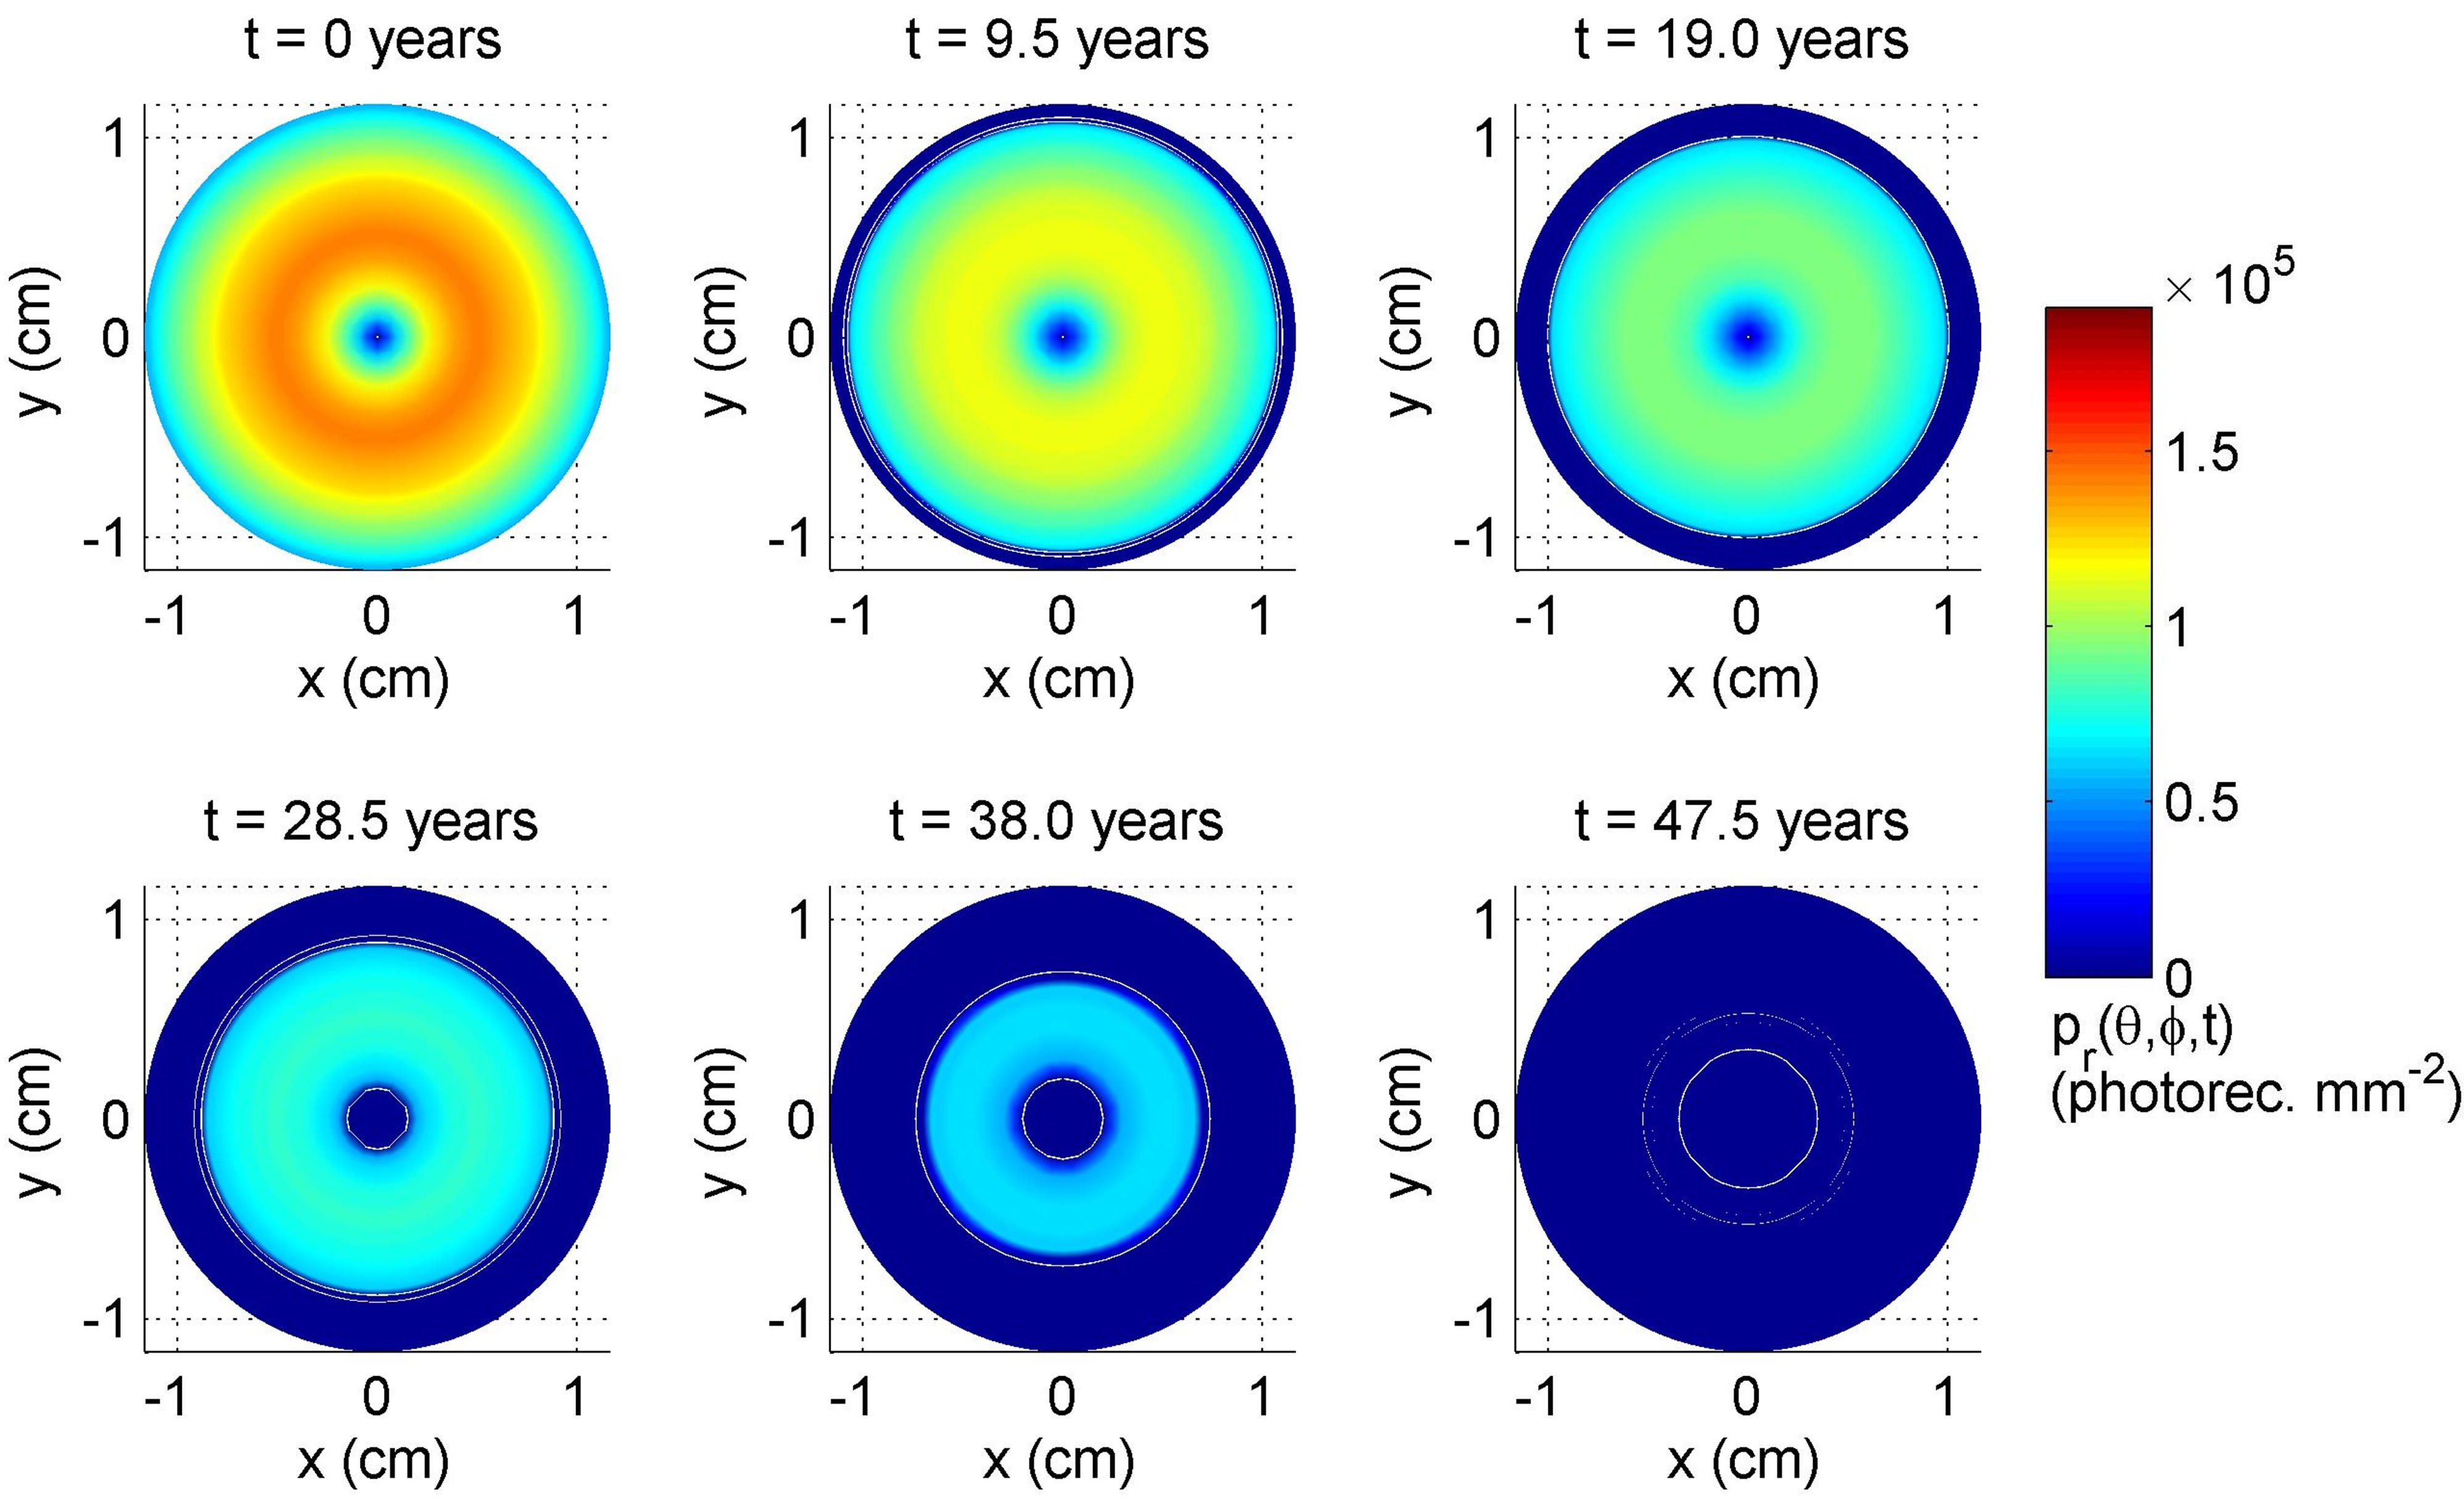
\includegraphics[scale=0.24]{Roberts_et_al_2018_Fig_5_a}
\end{center}
\caption{Exemplar spatio-temporal pattern of rod degeneration in RP, generated by the oxygen toxicity mechanism (the cone degeneration pattern is identical). The model replicates a classic pattern of retinal degeneration in RP, incorporating degeneration expanding inwards from the retinal periphery (ora serrata) and outwards from the parafoveal/perifoveal region. Figure reproduced, with permission, from \citet{Roberts_et_al_2018a}.}
\label{Fig_Roberts2018}
\end{figure}
%

Camacho et al. have constructed a range of well-mixed and compartmental ODE models, each exploring one or both of the trophic factor depletion and metabolic dysregulation hypothesis, under both healthy and RP conditions. Under healthy conditions, their models replicated the rhythmic variation in rod and cone outer segment length observed \emph{in vivo} \citep{Camacho_et_al_2010,Camacho_et_al_2016b,Colon_Velez_et_al_2003, Wifvat_et_al_2021}. Further, these models predicted conditions under which rods and cones can stably coexist, revealing that the assistance provided to the cones by the rods via a trophic factor is crucial in this respect \citep{Camacho_et_al_2010,Camacho_et_al_2016b,Colon_Velez_et_al_2003, Wifvat_et_al_2021}. This group’s retinal metabolic models are the most biochemically detailed to have been generated to date, using sensitivity and bifurcation analyses to determine which processes are most important in maintaining a healthy homeostasis \citep{Aparicio_et_al_2022,Dobreva_et_al_2022,Camacho_et_al_2019,Camacho_et_al_2021a}. Under RP conditions, their models clarify and elucidate the stages of retinal degeneration that may be traced on the road to complete atrophy, highlighting which processes must change to allow progression to the next stage \citep{Camacho_and_Wirkus_2013,Camacho_et_al_2016,Camacho_et_al_2016c}. Further, they apply optimal control theory to identify optimal treatment strategies under various constraints \citep{Camacho_et_al_2014,Camacho_et_al_2020}.

Lastly, Burns et al. have formulated a 1D hybrid model for the toxic substance hypothesis, containing both continuous-deterministic and discrete-stochastic elements \citep{Burns_et_al_2002}. This model is effective in capturing the initial patchy loss of photoreceptors observed in RP, and is also capable of replicating the exponential decline in photoreceptor numbers measured in RP mouse models \citep{Clarke_et_al_2000}.
%
\subsection{Non-neovascular AMD}\label{Sec_nnAMD}
%
The retinal disease age-related macular degeneration (AMD) can be divided into three stages: early, intermediate and late \citep{Ferris_et_al_2013}. The early and intermediate stages are distinguished by the development of pigmentary abnormalities and the size of cholesterol-rich deposits known as drusen (singular, druse) which form between the RPE and Bruch’s membrane (BrM – hard and soft drusen), and between the RPE and photoreceptors (reticular pseudodrusen/subretinal drusenoid deposits), while the late stage may be characterised as dry or wet \citep{Coleman_et_al_2008,Ferris_et_al_2013,Jager_et_al_2008,Wu_et_al_2022}. Non-neovascular AMD (nnAMD), considered in this section, consists of the early and intermediate stages, together with the dry form of the late stage \citep[][see \textcolor{red}{Section \ref{???}} on wet/neovascular AMD]{Ferris_et_al_2013}. In the dry late stage, the central retina and choroid degenerate in a process known as geographic atrophy \citep[GA,][]{Coleman_et_al_2008,Jager_et_al_2008,Ly_et_al_2016}.

A number of mechanisms have been suggested to drive nnAMD including oxidative stress, drusen accumulation, cholesterol accumulation and lipofuscin accumulation \citep{Ambati_and_Fowler_2012,Handa_et_al_2019}. Mathematical models have been developed to consider each of these mechanisms and this area has great potential for future modelling studies \citep{Handa_et_al_2019,Luthert_et_al_2018}.

\citet{Mazzitello_et_al_2009} and \citet{Family_et_al_2010} constructed a simple stochastic model for the accumulation of lipofuscin, a chemical which builds up within RPE cells and may eventually prove toxic to them \citep{Sparrow_and_Boulton_2005}. They capture the aggregation of  lipofuscin granules, though they do not link this to RPE cell death.

\citet{Zekavat_et_al_2017} and \citet{Scheepers_et_al_2020} have developed compartmental ODE models for drusen and cholesterol accumulation. The models capture features such as the build-up of drusen and their macrophage-mediated elimination, and determine regions of parameter space in which a healthy homeostasis may be maintained.

\citet{Linsenmeier_and_Zhang_2017} and \citet{McHugh_et_al_2019} have developed 2D and 3D PDE models (respectively) to predict the effects of soft and hard drusen upon retinal oxygen distribution (see Figure \ref{Fig_LinZhang2017}). It was found that it is the size of a druse, rather than the diffusivity of oxygen within a druse, which has the greatest effect on photoreceptor oxygenation, and that wide (soft) druse are more likely to cause photoreceptor hypoxia (oxygen starvation) than tall (hard) druse. Further, \citet{Vercellin_et_al_2021} have constructed a 2D PDE model predicting the effects of reduced blood flow on central retinal oxygenation, identifying the most vulnerable regions.
%
\begin{figure}
\begin{center}
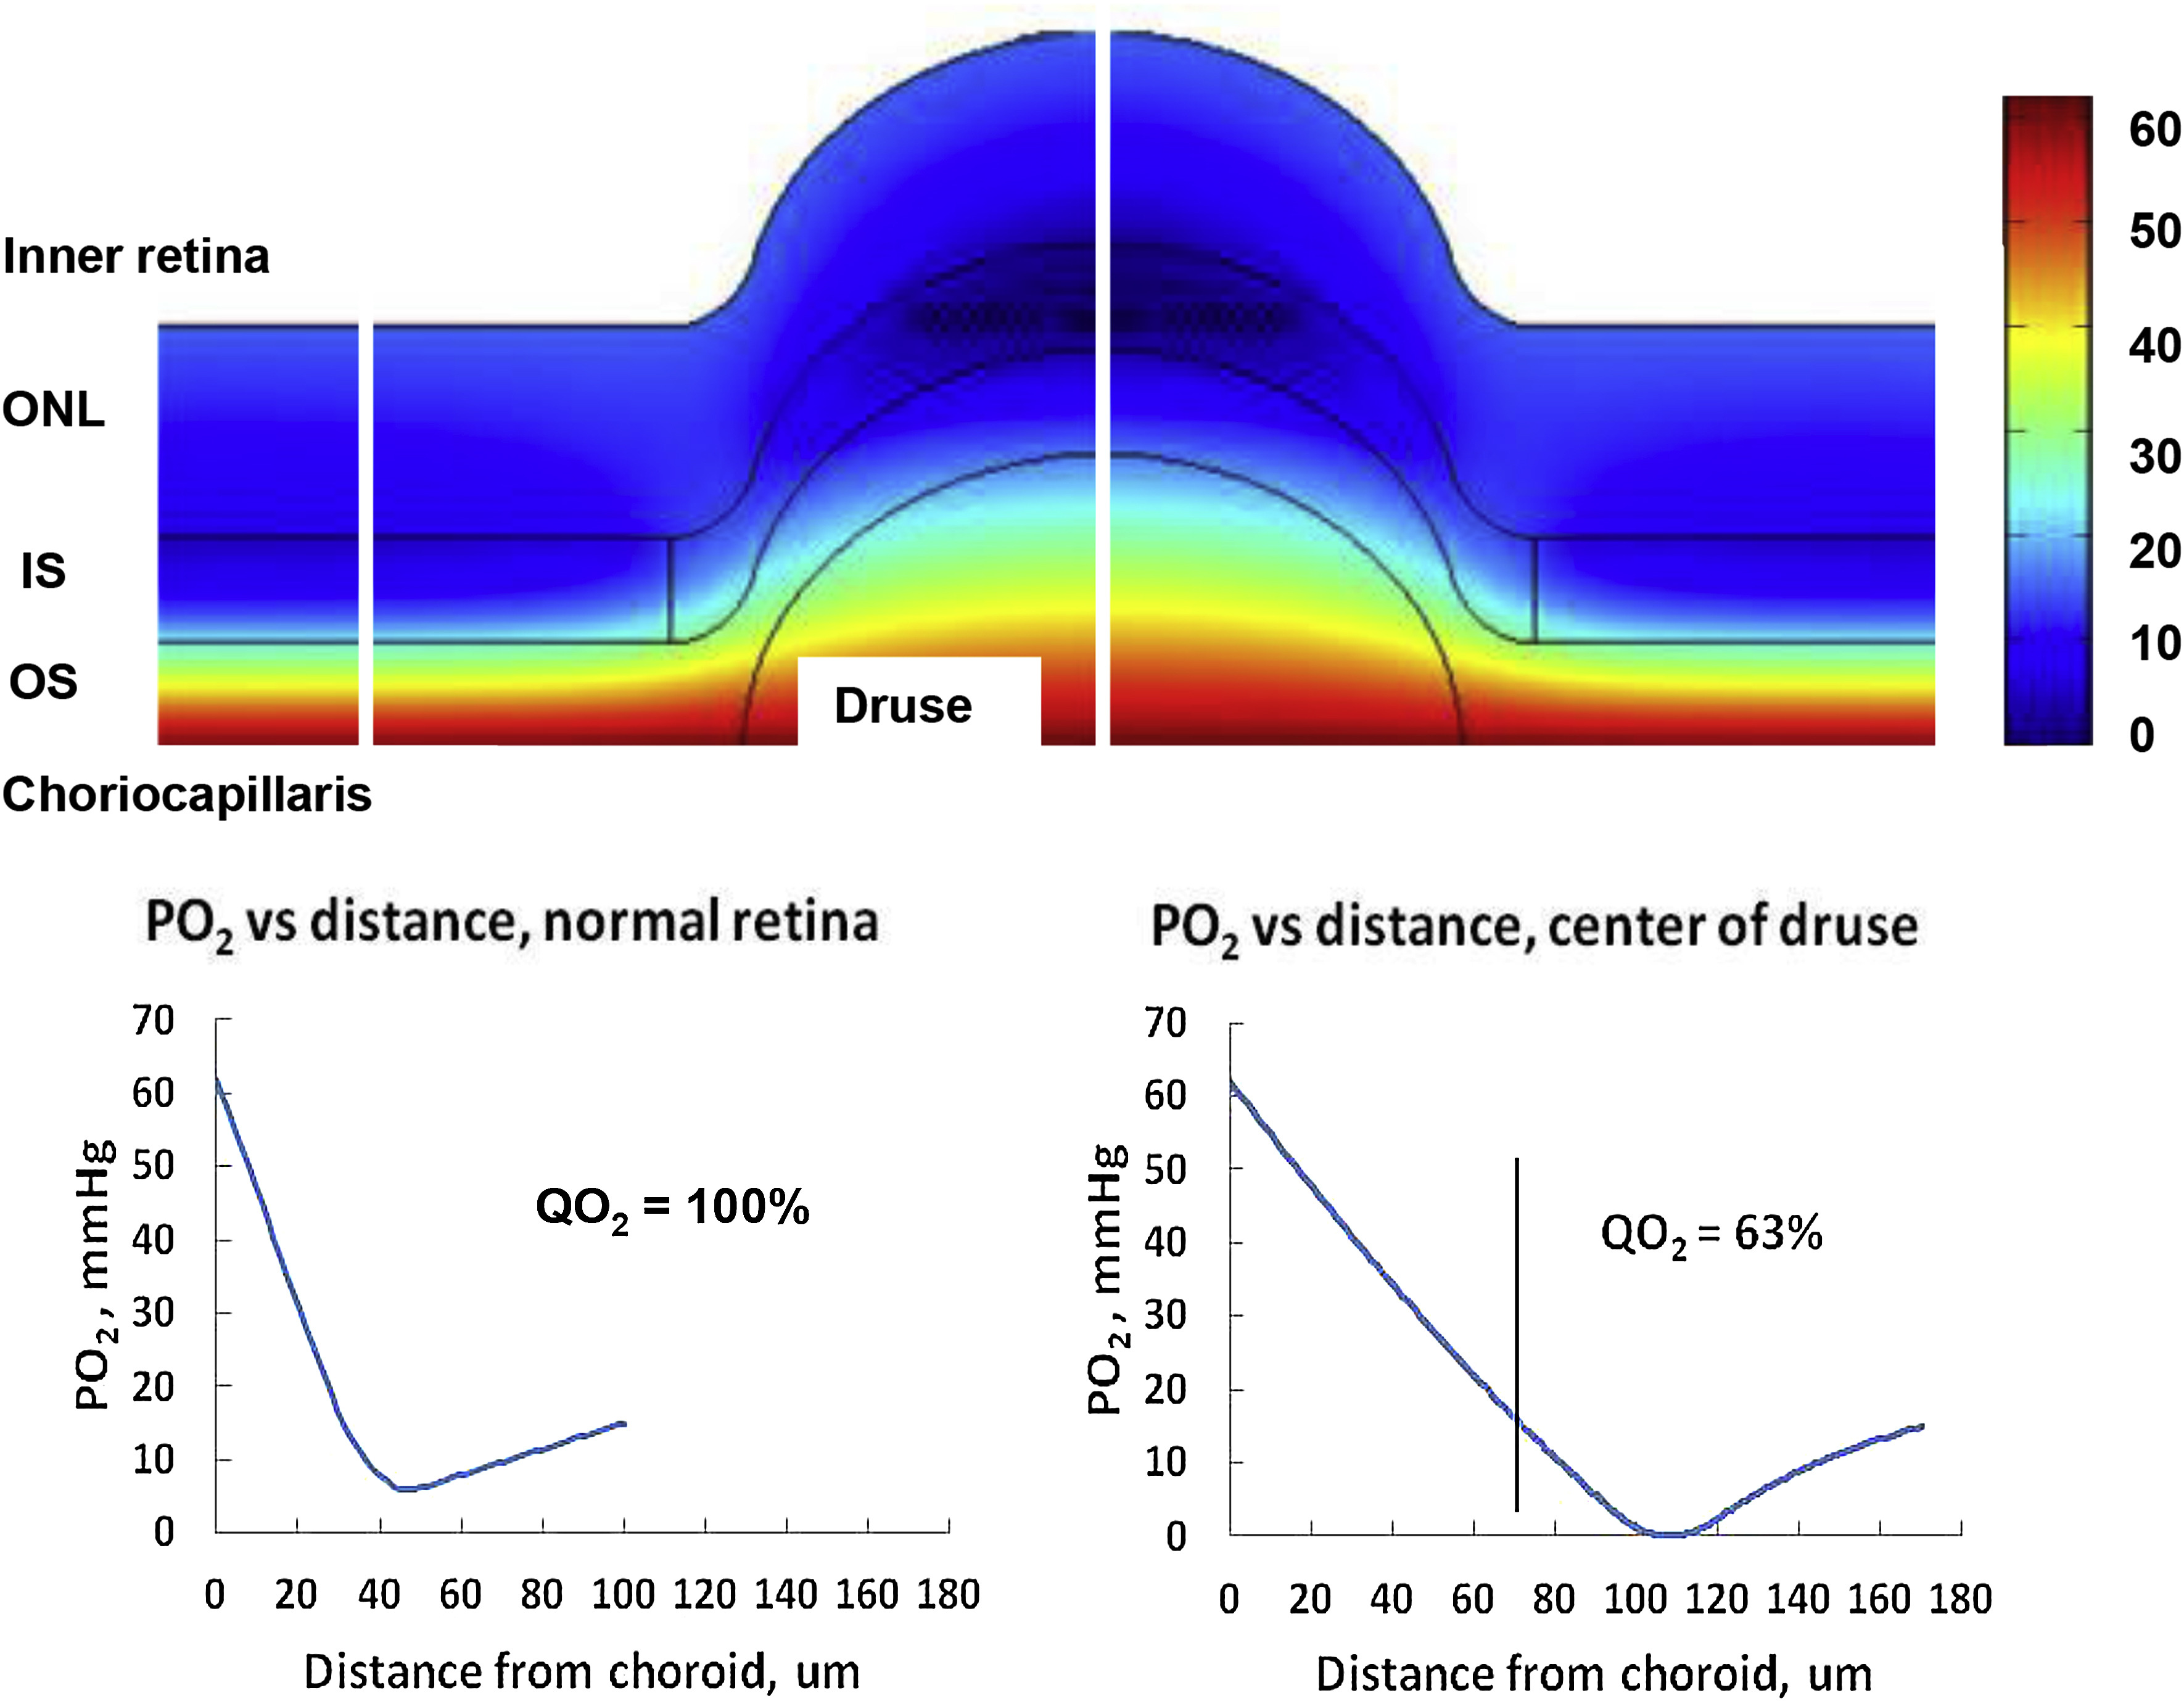
\includegraphics[scale=0.9]{Linsenmeier__and_Zhang_2017_Fig_21}
\end{center}
\caption{Oxygen profile (PO$_2$) through the outer retina in the presence of a large druse. Top panel: 2D heatmap showing the oxygen profile across normal and druse-containing retinal regions. Bottom panels: 1D profile through the normal (left) and druse-containing retinal regions (right). Figure reproduced, with permission, from \citet{Linsenmeier_and_Zhang_2017}. Abbreviations --- OS: outer segment, IS: inner segment, ONL: outer nuclear layer.}
\label{Fig_LinZhang2017}
\end{figure}
%

Lastly, \citet{Shen_et_al_2020} formulated a simple phenomenological model to predict GA progression based upon measurements of GA propagation rates within the literature. The model is successful in replicating some of the patterns seen \emph{in vivo}, though it is not capable of explaining the mechanisms behind these patterns.
%
%
\newpage
%
\bibliography{Paul_PBERev_Ref_NewVersion_Draft_1}{}
\bibliographystyle{elsarticle-harv}
%
\end{document}